\documentclass[10pt,a4paper]{article}
\usepackage[utf8]{inputenc}
\usepackage[spanish]{babel}
\usepackage{amsmath}
\usepackage{amsfonts}
\usepackage{amssymb}
\usepackage{graphicx}
\usepackage{algorithm2e}
\author{Markus Fischer • Guzmán López • David Pérez • Ander Raso}
\title{Proyecto de Minería de Datos: \linebreak Clustering aplicado a Autopsias Verbales}

\date{}

%Borrador de la memoria completa: estructura con todas las secciones y en cada sección esquema del contenido
%
%    1. Introducción completa
%        1.1 En qué consiste la tarea
%        1.2 Qué retos presenta
%        1.3 Propuesta para abordarlos
%    2. Descripción y análisis de datos completo
%    3. Pre-proceso: describir en qué consiste, fase de limpieza de datos, qué rutinas se han aplicado para cambiar el formato de datos de texto a un vector numérico
%    4. Clustering: Algoritmo de clustering en pseudo-código.
%    5. Evaluación: ¿Qué técnicas de evaluación se emplearán? Detallar formalismo teórico
%    6. Detalle de los experimentos que se van a realizar y el objetivo de cada experimento
%    7. Conclusiones y trabajo futuro: vacío hasta completar trabajo
%    8. Bibliografía

\begin{document}
\maketitle
\pagenumbering{gobble}

\newpage
\pagenumbering{arabic}
\tableofcontents

\newpage
\section{Introducción}
	\subsection{Objetivo de la tarea}
	\paragraph{}
	En este proyecto se nos encarga la tarea de trabajar en el campo del \textit{Text Mining} y del \textit{clustering} de documentos. Nuestro objetivo consiste en realizar una clasificación no supervisada de una gran cantidad de textos. La clasificación no supervisada consiste en agrupar las instancias en distintos grupos, o clusters, según su similitud. Se intenta conseguir que las instancias de un cluster determinado sean similares entre sí a la vez que distintas de las instancias que no pertenecen al cluster.

	\subsection{Propuesta de trabajo del grupo}
	\paragraph{}
	Como grupo, hemos decidido realizar la tarea sobre la colección de autopsias verbales que se nos propuso como una de las posibles opciones. Esto se debe a que, además de considerar el tema muy interesante, creemos que es una propuesta que se encuentra muy próxima al uso que se da al \textit{Text Mining} en el ámbito científico.
	\paragraph{}
    Sin embargo, de esta decisión también surgen ciertos retos a los que debemos poner solución:
	\begin{itemize}
		\item Muchos de los reportes de autopsia están en un lenguaje poco preciso y muchas veces ininteligible, probablemente causado tanto por el desconocimiento de los que dieron el reporte, como por las traducciones que se han hecho a estos.
		\item En muchas ocasiones no hay reporte verbal o este es irrelevante, por lo que la única información útil de que se dispone es de los datos del difunto, tales como país, edad, sexo, etc.
		%TODO: Añadir alguna más para que no quede vacío.
	\end{itemize}

\section{Descripción y análisis de datos}
	\paragraph{}
	En este proyecto vamos a trabajar con autopsias verbales. Estas son reportes que dan familiares o personas cercanas a un fallecido en lugares donde, por norma general, no se realiza una autopsia post-mortem a menos que sea estrictamente necesario. Estas autopsias se componen de información básica del paciente (edad, sexo, etc.) así como del reporte oral que ha dado el relativo al que se ha entrevistado.
	\paragraph{}
	La base de datos de las autopsias verbales se compone de casi 12000 instancias. En cada instancia disponemos de una serie de atributos:

	\begin{itemize}
		\item \textbf{newid:} Identificador numérico de la instancia.
		\item \textbf{module:} Grupo de edad del fallecido. Los valores posibles son ``neonate'', ``child'' y ``adult'' (Fig: \ref{fig:age_graph}).
		\item \textbf{site:} Lugar del que proviene la autopsia: los valores posibles para este campo son (Fig: \ref{fig:loc_graph}):
	    \begin{itemize}
		    \item AP=Andhra Pradesh, India
		    \item Dar=Dar es Salaam, Tanzania
		    \item UP=Uttar Pradesh, India
		    \item Pemba=Pemba, Tanzania
		    \item Bohol=Bohol, Philippines
		    \item Mexico=Distrito Federal, Mexico
	    \end{itemize}

		\begin{figure}
			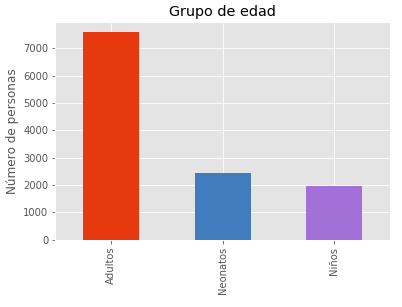
\includegraphics[width=\linewidth]{figures/plot_grupo_edad.png}
			\caption{Número de instancias según la edad del fallecido}
			\label{fig:age_graph}
		\end{figure}

		\begin{figure}
			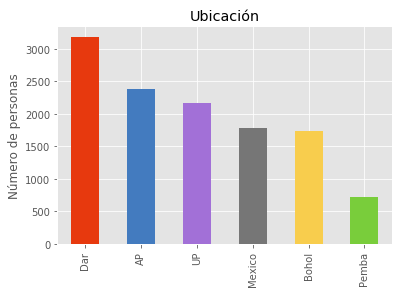
\includegraphics[width=\linewidth]{figures/plot_ubicacion.png}
			\caption{Número de instancias según la ubicación del fallecido}
			\label{fig:loc_graph}
		\end{figure}

		\begin{figure}
			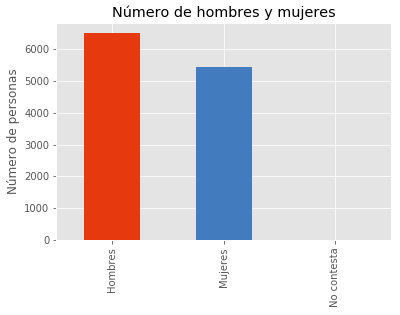
\includegraphics[width=\linewidth]{figures/plot_sexo.png}
			\caption{Número de instancias según el sexo del fallecido}
			\label{fig:sex_graph}
		\end{figure}

		\item \textbf{gs\_text34:} Causa de la muerte del paciente.
		\item \textbf{sex:} Sexo del difunto. Los valores posibles son 1, 2, 3 y 4. Cada uno de estos valores hace referencia a ``hombre'', ``mujer'', ``se niega a responder'' y ``desconocido'' respectivamente (Fig: \ref{fig:sex_graph}).
		\item \textbf{age\_years:} Edad del fallecido en años. En caso de ser igual a 999 significa que es desconocida.
		\item \textbf{age\_months:} Edad del fallecido en meses. En caso de ser igual a 99 significa que es desconocida.
		\item \textbf{age\_days:} Edad del fallecido en días. En caso de ser igual a 99 significa que es desconocida.
		\item \textbf{open\_response:} Declaración de la persona cercana al difunto en caso de que hubiese una. En este texto se han eliminado todas las referencias que se diesen en la declaración que pudiesen relacionarse con el difunto para asegurar su privacidad, tales como menciones a los lugares y hospitales en los que se ha encontrado, el nombre de personas o fechas concretas en relación al fallecido, etc. En su lugar se han sustituido por palabras neutrales entre corchetes, tales como ``[PERSON]'' o ``[HOSPITAL]''.
	\end{itemize}

\section{Preproceso de datos}
	\paragraph{}
	El formato original del archivo de autopsias es un xlsx, es decir, una hoja de cálculo de Microsoft Office. Esto nos facilita mucho la tarea de procesar los textos, ya que es muy fácil convertir de xlsx a formatos de texto plano. En nuestro caso elegimos csv, ya que es un formato muy limpio, fácil de entender y compatible con gran parte de las librerías que vamos a utilizar.

	\subsection{Limpieza de textos}
	\paragraph{}
	Una vez tenemos nuestro documento como csv, procedemos a preprocesarlo. Ya que los valores de identificador, grupo de edad, lugar, diagnóstico, sexo y edad están codificados según unos criterios que se mantienen a lo largo de todas las instancias, sabemos que no debemos preprocesarlos. Sin embargo, en el campo de la respuesta verbal sí que tenemos que solucionar algunas anomalías:

	\begin{itemize}
		\item \textbf{Mayúsculas y minúsculas:} Para evitar diferencias entre palabras escritas completamente en minúscula, completamente en mayúscula o con la primera letra mayúscula, debemos transformar todas ellas a un mismo formato. En nuestro caso el formato escogido son las minúsculas.
		\item \textbf{Saltos de línea:} En algunos casos nos encontramos con saltos de línea internos en el texto. Ya que csv separa sus diferentes atributos por comas y las instancias por líneas, los saltos de línea internos en el texto crean inconsistencias y errores al procesar el csv. El método más fácil para deshacerse de ellos pero mantener el texto en el mismo formato es sustituirlos por espacios.
		\item \textbf{Números:} Los números, pese a ser uno de los elementos más comunes en los textos, han sido uno de los más difíciles de preprocesar, no por su dificultad en cuanto a programar, sino a la decisión que tomar en cuanto a ellos. Esto se debe a que se toman como una palabra por si mismos y pese a tener un peso informativo alto, sólo es así cuando va acompañado de otra palabra a la que calificar. Ya que los programas de \textit{Text Mining} los van a considerar independientes del resto de palabras, hemos considerado que la información que van a aportar es suficientemente baja como para simplemente eliminarlos del texto.
		\item \textbf{Tokens:} Se consideran tokens a todas las palabras recurrentes que no tienen ni significado ni peso informativo, como por ejemplo ``the'' o ``a''. Mediante un diccionario de tokens en la lengua inglesa hemos podido detectar todos ellos y eliminarlos del texto.
		\item \textbf{Símbolos:} Aquí tenemos varios problemas que debemos arreglar de diferentes formas.
		\begin{itemize}
			\item \textbf{Barras ``/'':} En ocasiones nos encontramos con dos palabras escritas de modo "palabra1/palabra2". Para evitar que se procesen ambas como una misma palabra, realizamos el mismo procedimiento que utilizamos con los saltos de línea: cambiamos las barras por espacios.
			\item \textbf{Corchetes ``[ ]'':} En gran parte de las instancias que disponen de autopsia verbal nos encontramos con referencias a nombres de personas, hospitales, años concretos, etc. Para preservar la privacidad de los fallecidos y sus relativos estos han sido sustituidos por sus correspondientes palabras clave entre corchetes, como por ejemplo ``[PATIENT]'' o ``[HOSPITAL]''. Ya que estos datos son en la inmensa mayoría de casos de poca utilidad, hemos decidido que estás palabras serán completamente eliminadas de los textos.
		\end{itemize}
	\end{itemize}

	\subsection{\textit{Word vector}}
	\paragraph{}
	Después de limpiar los textos de las instancias necesitamos convertir ese texto a un formato que podamos utilizar. El formato escogido es el TF-IDF, el cual consiste en una representación vectorial del conjunto de palabras presentes en todos los documentos (instancias). Cada una de las palabras se evalúa individualmente y se le asigna un valor numérico en función al número de apariciones que tiene en cada documento, pero teniendo en cuenta también en cuántos de los documentos aparece para evitar darle excesiva importancia a palabras que simplemente se repiten por ser comunes.
	La definición matemática es: 
		\begin{equation}
	tf(t,d)=\frac{f(t,d)}{max[f(t,d):t \in d]}
	\end{equation}
	\begin{itemize}
	    \item t: término
	    \item d: documento
	\end{itemize}
	\begin{equation}
	idf(t,D)=\log \frac{|D|}{[d \in D : t \in d]}
	\end{equation}
	\begin{itemize}
	    \item D: Numero de documentos en la colección
	\end{itemize}
	\begin{equation}
	TFIDF(t,d,D)=tf(t,d) \dot idf(t,D)
	\end{equation}
	\paragraph{}
	Escogimos la representación TF-IDF en favor de \textit{Bag of Words} por el hecho de que aporta más información. \textit{Bag of Words} se limita a indicar la presencia o ausencia de palabras en los documentos mientras que TF-IDF le asigna un valor en función de su aparente importancia teniendo en cuenta todos los documentos.

\section{Clustering}
	\paragraph{}
	Para el \textit{clustering} hemos decidido utilizar el algoritmo \textit{k-means clustering}, el cual implementaremos en Python. Algunas de las opciones para el algoritmo a tener en cuenta son:
	\begin{itemize}
		\item \textbf{Inicialización de los centroides:} Hay varias formas de elegir los valores iniciales de los centroides, y su inicialización podría tener repercusión en los resultados.
		\begin{itemize}
		    \item \textbf{Inicialización a instancias aleatorias: } cada centroide se toma el valor de una instancia elegia aleatoriamente. En nuestro caso los inicializamos de esta manera.
		    \item \textbf{Inicialización a partir de un \textit{clustering} previo:} Se realiza una agrupación preliminar a $2k$ clusters. De esos clusters se eligen los $k$ que más separados estén para la inicialización.
	    \end{itemize}
		\item \textbf{Cálculo de las distancias:} La fórmula utilizada para calcular la distancia será la distancia Minkowski, con \(m \in \Re\). \(m=1\) es la distancia Manhattan y \(m=2\) es la distancia Euclídea.
		Cálculo de la distancia con Minkowski \cite{Minkowski}: 
		    \begin{equation}
		    	 D(X,Y)=(\sum_{i=1}^n |x_i - y_i|^m)^\frac{1}{m}
			\end{equation}		    
		    $D$: distancia \newline
		    $x$, $y$: vectores  \newline
		    $m$: orden (normalmente 1 o 2 para las distancias Manhattan o Euclídea respectivamente)\newline
		En el caso concreto del cálculo de la distancia segun Manhattan (\(m=1\)) \cite{Minkowski}:
		\begin{equation}
		    D(X,Y)=\sum_{i=1}^n |x_i - y_i|
		\end{equation}
		
		\item \textbf{Definición de distancia \textit{inter-cluster}:} También existen varias formas para buscar la distancia entre dos clusters distintos. En este caso, vamos a trabajar con dos:
		\begin{itemize}
		    \item \textit{Complete-link}. La distancia entre dos clusters es igual a la distancia entre las dos instancias, una de cada cluster, más lejanas entre sí.
		    \begin{equation}
		    d(C_i,C_j)=\smash{\displaystyle\max_{ \forall x^{(r)}\in C_i ; \forall x^{(s)} \in C_j}} d(x^{(r)},x^{(s)})
	    	\end{equation}
		    \item \textit{Single-link}. La distancia d entre dos clusters (C$_i$, C$_j$) es igual a la distancia entre las dos instancias (x$^{(r)}$,x$^{(s)}$), una de cada cluster, más cercanas entre sí.
		    \begin{equation}
		    d(C_i,C_j)=\smash{\displaystyle\min_{\forall x^{(r)}\in C_i ; \forall x^{(s)} \in C_j}} d(x^{(r)},x^{(s)})
		    \end{equation}
		    \item \textit{Average-link}. La distancia entre dos clusters (C$_i$, C$_j$) es igual a la distancia entre los centroides (m$_i$,m$_j$) de cada cluster. \cite{AliciaPerez}

		    \begin{equation}
		    d(C_i,C_j)=d(m_i,mj) \text{  para  } m_i=\frac{1}{|C_i|}\sum_{\forall x^{(r)} \in C_i} x^{(r)}  
	    	\end{equation}
	    \end{itemize}
	    \item \textbf{Criterio de convergencia:} Parámetro para decidir cuándo dar por finalizado el algoritmo de \textit{clustering}. Terminamos éste cuando la variación de los centroides sea más pequeña que nuestro umbral de una iteración a la siguiente. También tenemos un número máximo de iteraciones tras las cuales el algoritmo termina forzosamente, para evitar posibles ciclos.
	\end{itemize}

	\begin{algorithm}
		\SetAlgoLined
		\SetKwInOut{Input}{input}
		%\SetKwInOut{Output}{output}
		
		\Input{Conjunto de instancias $\mathrm{X}$}
		%\Output{A partition of the bitmap}
		\BlankLine
		\tcp{inicializar los $k$ centroides}
		inicializar $m_i, i \in [1, k]$\;
		$terminado \leftarrow False$\;
		\While{no terminado}{
			\tcp{para cada instancia, activar el bit correspondiente al centroide más cercano}
			\ForEach{$x^t \in \mathrm{X}$}{
				\eIf{$\|x^t - m_i\| = min_j\|x^t - m_i\|$}{
					$b^t_i \leftarrow 1$\;
				}{
					$b^t_i \leftarrow 0$\;
				}		
			}
			\tcp{guardar los centroides anteriores para comparación}
			$n \leftarrow m$\;
			\tcp{actualizar los nuevos centroides como la media de todas sus instancias}
			\ForEach{$m_i, i \in [1, k]$}{
				$m_i \leftarrow \sum_{t} b^t_i x^t / \sum_{t} b^t_i$\;
			}
			\tcp{comprobar convergencia de los centroides}
			\If{$\|n - m\| < threshold$}{
				$terminado \leftarrow True$\;
			}
		}
		\caption{Algoritmo \textit{k-means clustering} (pseudocódigo)}
	\end{algorithm}

	\subsection{Representación gráfica}
	\paragraph{}
	Una vez que tenemos las instancias separadas en clusters, sería interesante representarlas gráficamente para poder ver como se relacionan los clusters, calculados a partir del texto describiendo la enfermedad, con la causa de la muerte anotada en las autopsias. Para ello, tenemos que reducir el enorme espacio de atributos de las instancias a algo que podamos representar en un espacio de no más de tres dimensiones. Para ello pensamos en utilizar el método PCA (\textit{Principal Components}) el cual reduce un gran número de variables a una serie de valores representativos, ortogonales entre sí para representarlos en espacios de pocas dimensiones. Con este método podemos convertir nuestras instancias con cerca de 8000 atributos a dos atributos cada una para poder representarlas en un plano cartesiano.

\section{Evaluación}
	\paragraph{}
	Para evaluar el modelo obtenido vamos a utilizar la métrica de SSE (\textit{Sum of Square Errors}). Para cada uno de los clusters calculamos el error (distancia) cuadrático de cada instancia con respecto al centroide, y sumando todos estas distancias obtenemos el SSE total del cluster; su cohesión.
	\begin{equation}
		SSE(C_i) = \sum_{x \in C_i} d^2(x, c_i)
	\end{equation}
	\paragraph{}
	De la misma forma, sumando el SSE de cada cluster podemos obtener la cohesión total de la partición.
		$$C = \{C_1, C_2, C_3, ..., C_k\}$$
	\begin{equation}
		SSE(C) = \sum^{k}_{i=1} SSE(C_i) = \sum^{k}_{i=1} \sum_{x \in C_i} d^2(x, c_i)
	\end{equation}
	Para comparar cohesión entre clusters, calcularemos primero el SSE medio de los clusters, dividiendo el SSE de cada uno entre el número de instancias que contiene, ya que los clusters más poblados tendrán, por lo general, un SSE mayor solamente por su alto número de instancias, independientemente de su cohesión.
	
\section{Experimentos}
	\paragraph{}
	Como experimentos vamos a realizar el clustering con distintos valores en los principales parámetros: k (número de clusters a crear), m (parámetro para la distancia Minkowski) y la estrategia de inicialización de centroides.
	
	\subsection{Resultados}	
	\subsubsection{Parámetro k}
	\paragraph{}
	Hemos probado a hacer el clustering con dos valores distintos de k: 48 y 96. En los datos hay un total de 46 causas de muerte registradas por lo que decidimos crear, por un lado, tantos clusters como clases, y, por otro, el doble, para ver si había alguna diferencia notable.
	\begin{figure}
		\centering
		\makebox[\columnwidth]{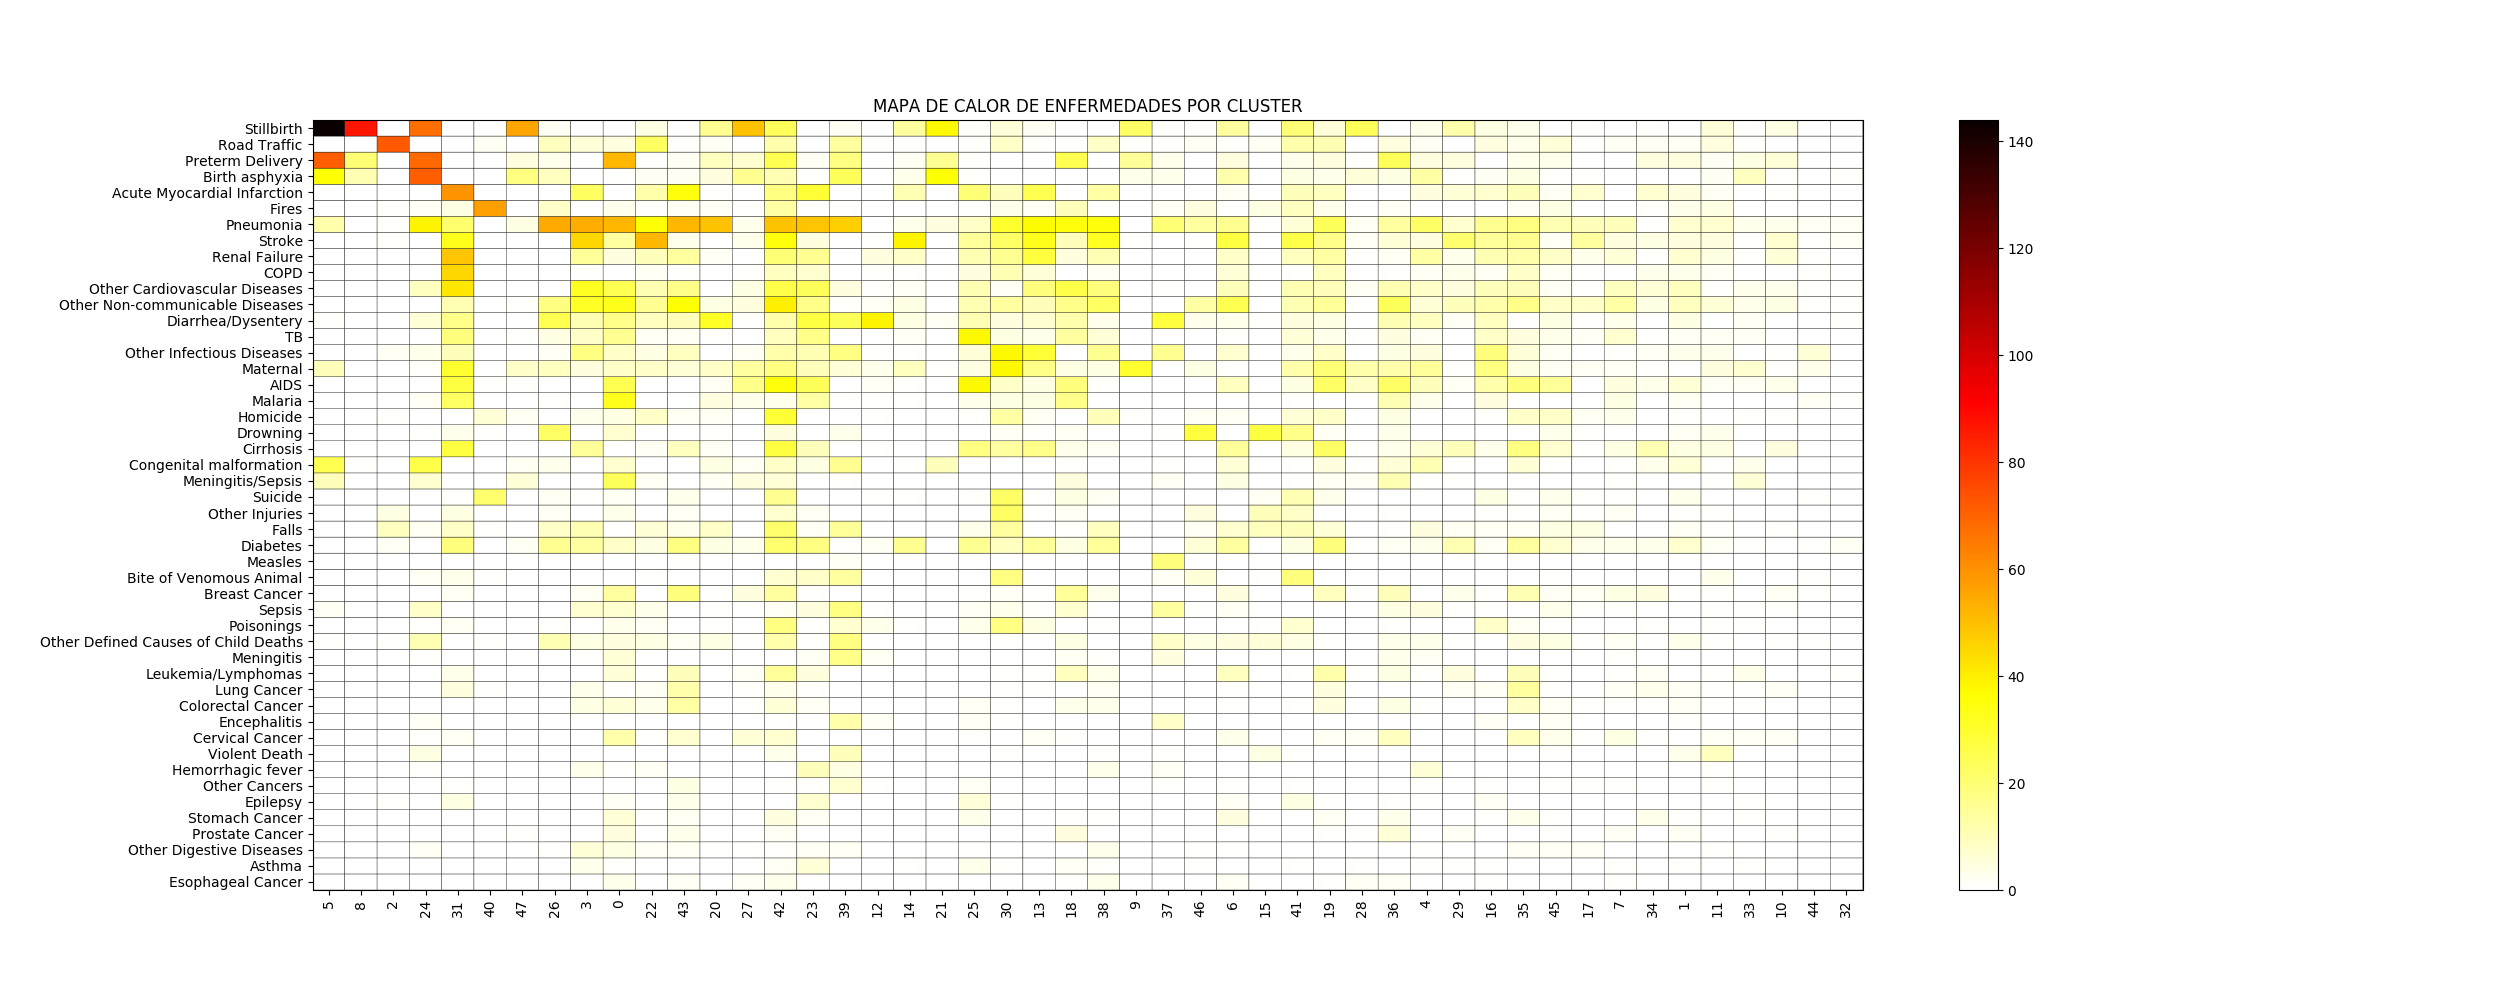
\includegraphics[width=\paperwidth]{figures/heatmap_k48_m2_initrandom.png}}
		\caption{Heatmap (k=48, m=2, init=random)}
		\label{fig:htm_48_2_random}
	\end{figure}
	\begin{figure}
		\centering
		\makebox[\columnwidth]{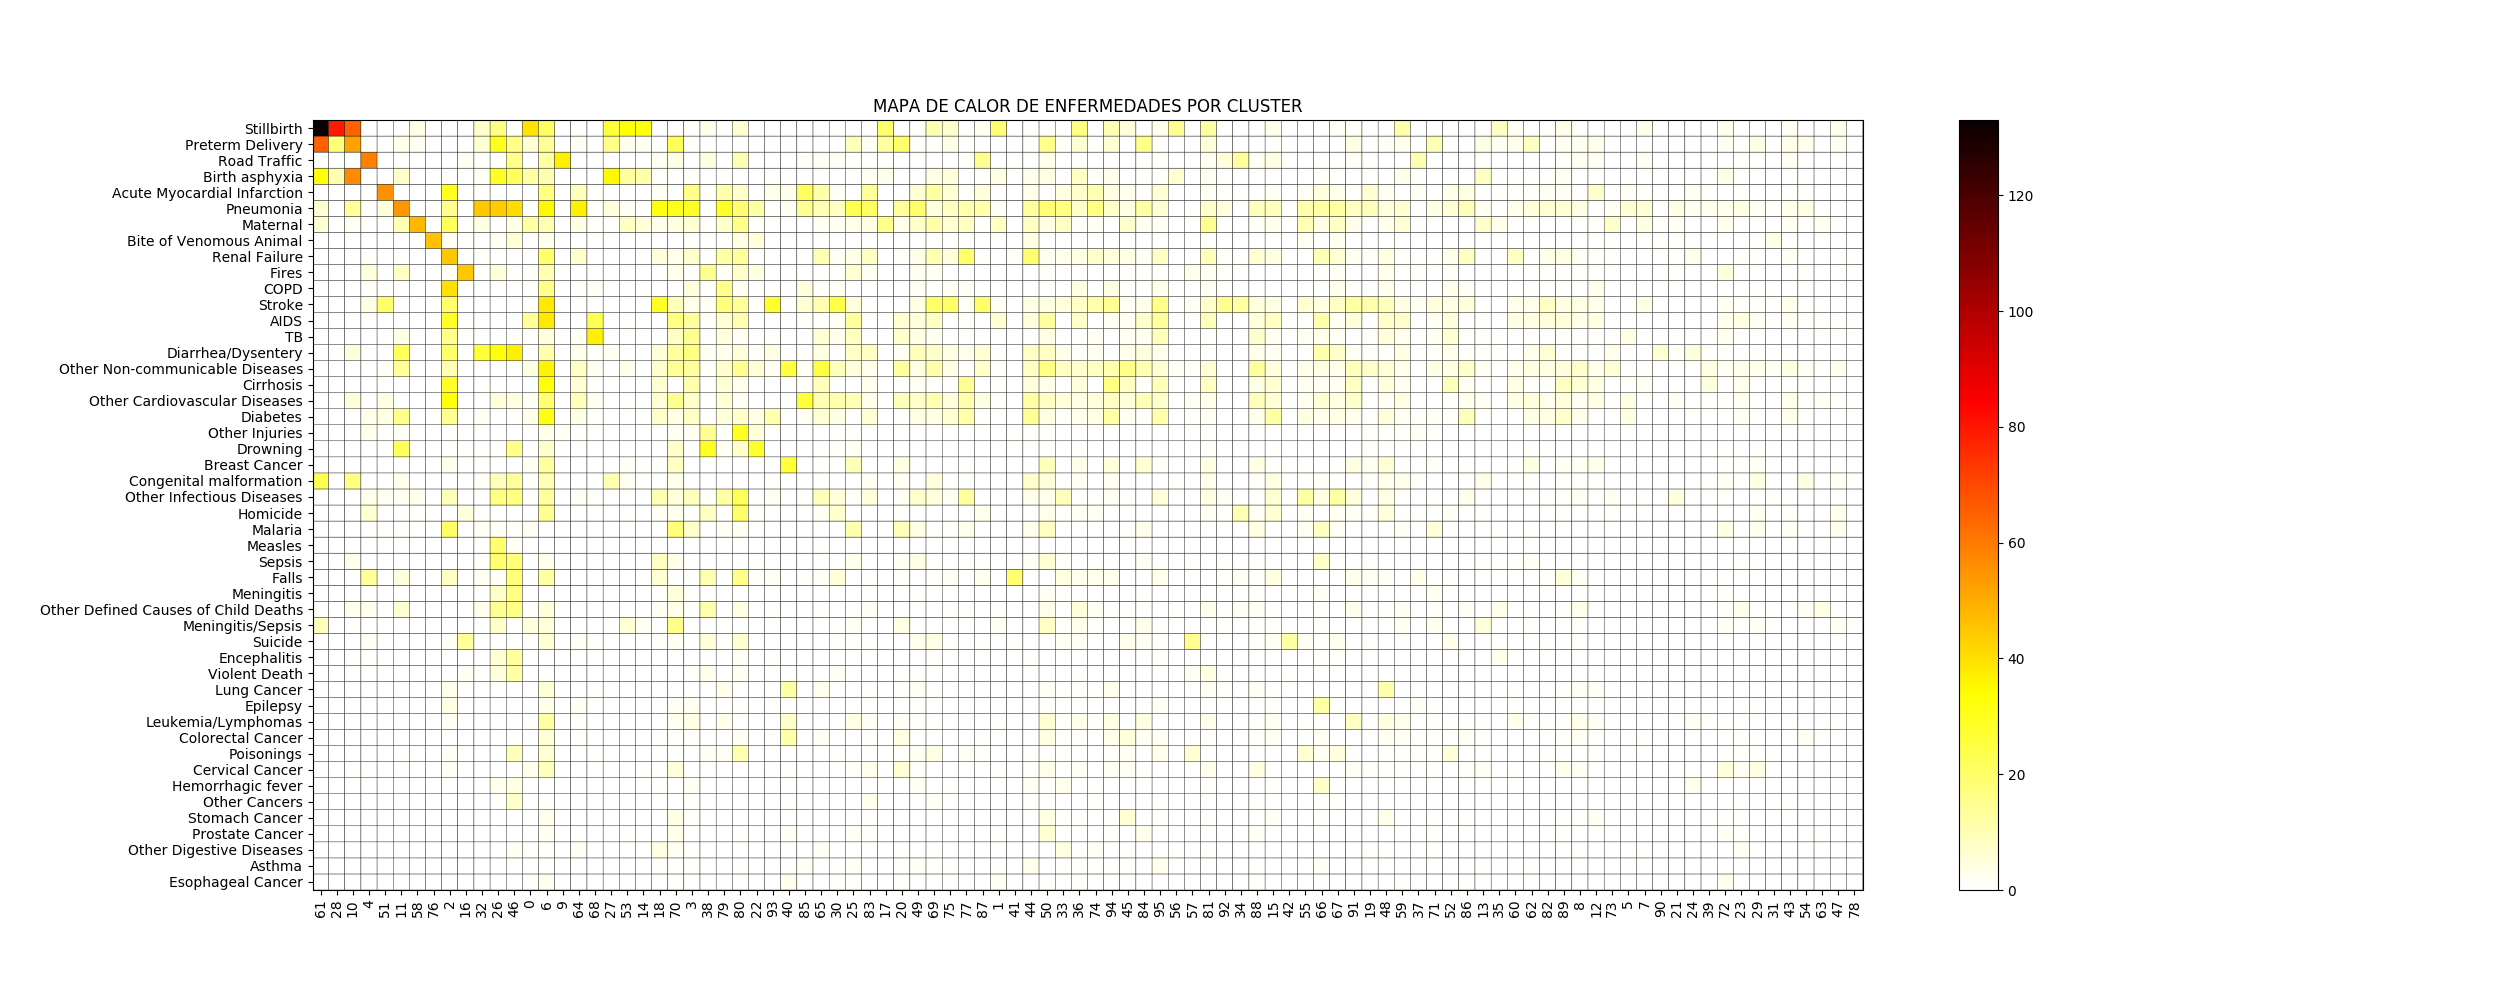
\includegraphics[width=\paperwidth]{figures/heatmap_k96_m2_initrandom.png}}
		\caption{Heatmap (k=96, m=2, init=random)}
		\label{fig:htm_96_2_random}
	\end{figure}
	
	\paragraph{}
	No resultó haber gran diferencia en los SSE medios de los clusters, pero mirando a los heatmaps de las particiones (Fig: \ref{fig:htm_48_2_random} y \ref{fig:htm_96_2_random}) se puede notar como la relación entre cluster y causa de muerte está bastante más dispersa cuando tenemos solo 48 clusters que cuando tenemos 96.
	
	\subsubsection{Inicialización de centroides}
	\paragraph{}
	Los dos métodos de inicialización que hemos probado son, inicialización aleatoria e inicialización a partir de una partición anterior de 2k clusters, de los cuales se eligen los k clusters más separados entre sí.
	\paragraph{}
	Comparando los resultados, para los dos casos el SSE medio por cluster es similar, sin embargo el SSE total por cluster es considerablemente distinto. En la inicialización aleatoria los clusters con mayor SSE tiene menos error que sus contrarios, mientras que en el otro extremo, los clusters de inicialización aleatoria con menor SSE tienen más error que los de inicialización a partir de partición previa. Esto se debe a que la densidad de instancias está más centralizada en la inicialización 2k que en la aleatoria; hay más clusters con muchas instancias y más clusters con pocas.
	\begin{figure}
		\centering
		\makebox[\columnwidth]{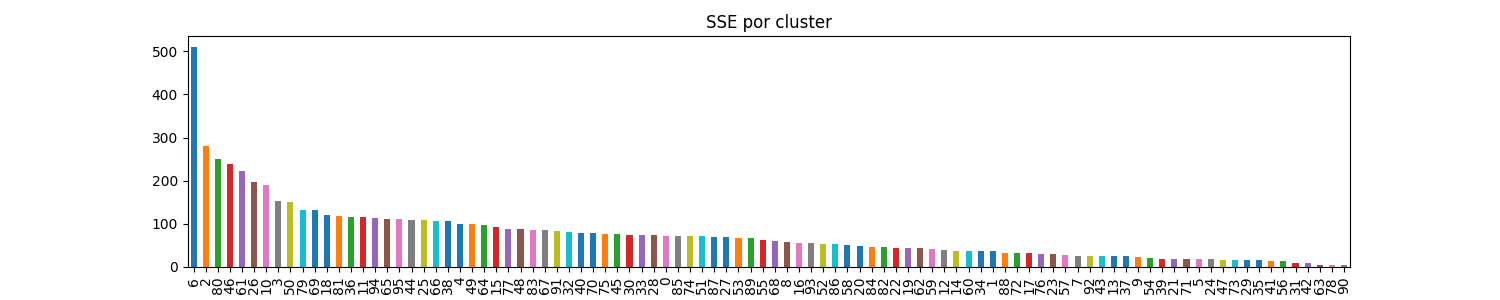
\includegraphics[width=\paperwidth]{figures/sse_plot_k96_m2_initrandom.png}}
		\caption{SSE por cluster (k=96, m=2, init=random)}
		\label{fig:sse_96_2_random}
	\end{figure}
	\begin{figure}
		\centering
		\makebox[\columnwidth]{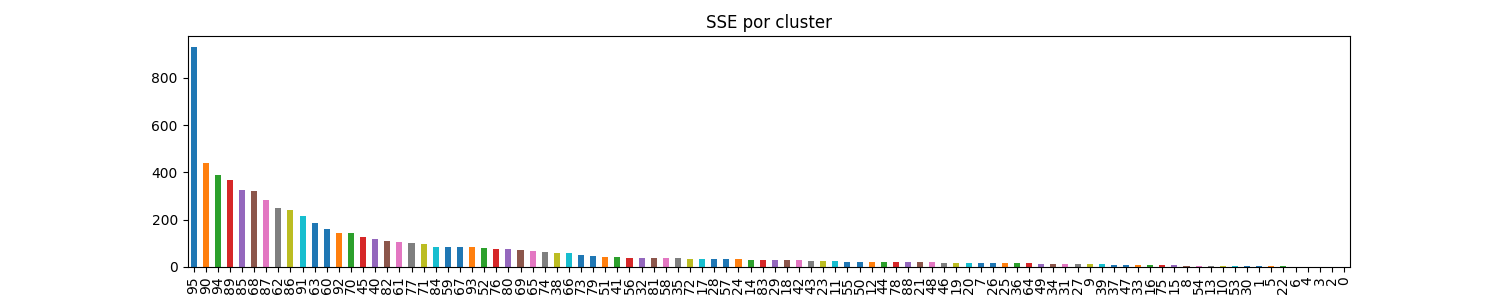
\includegraphics[width=\paperwidth]{figures/sse_plot_k96_m2_init2k.png}}
		\caption{SSE por cluster (k=96, m=2, init=2k)}
		\label{fig:sse_96_2_2k}
	\end{figure}
	\begin{figure}
		\centering
		\makebox[\columnwidth]{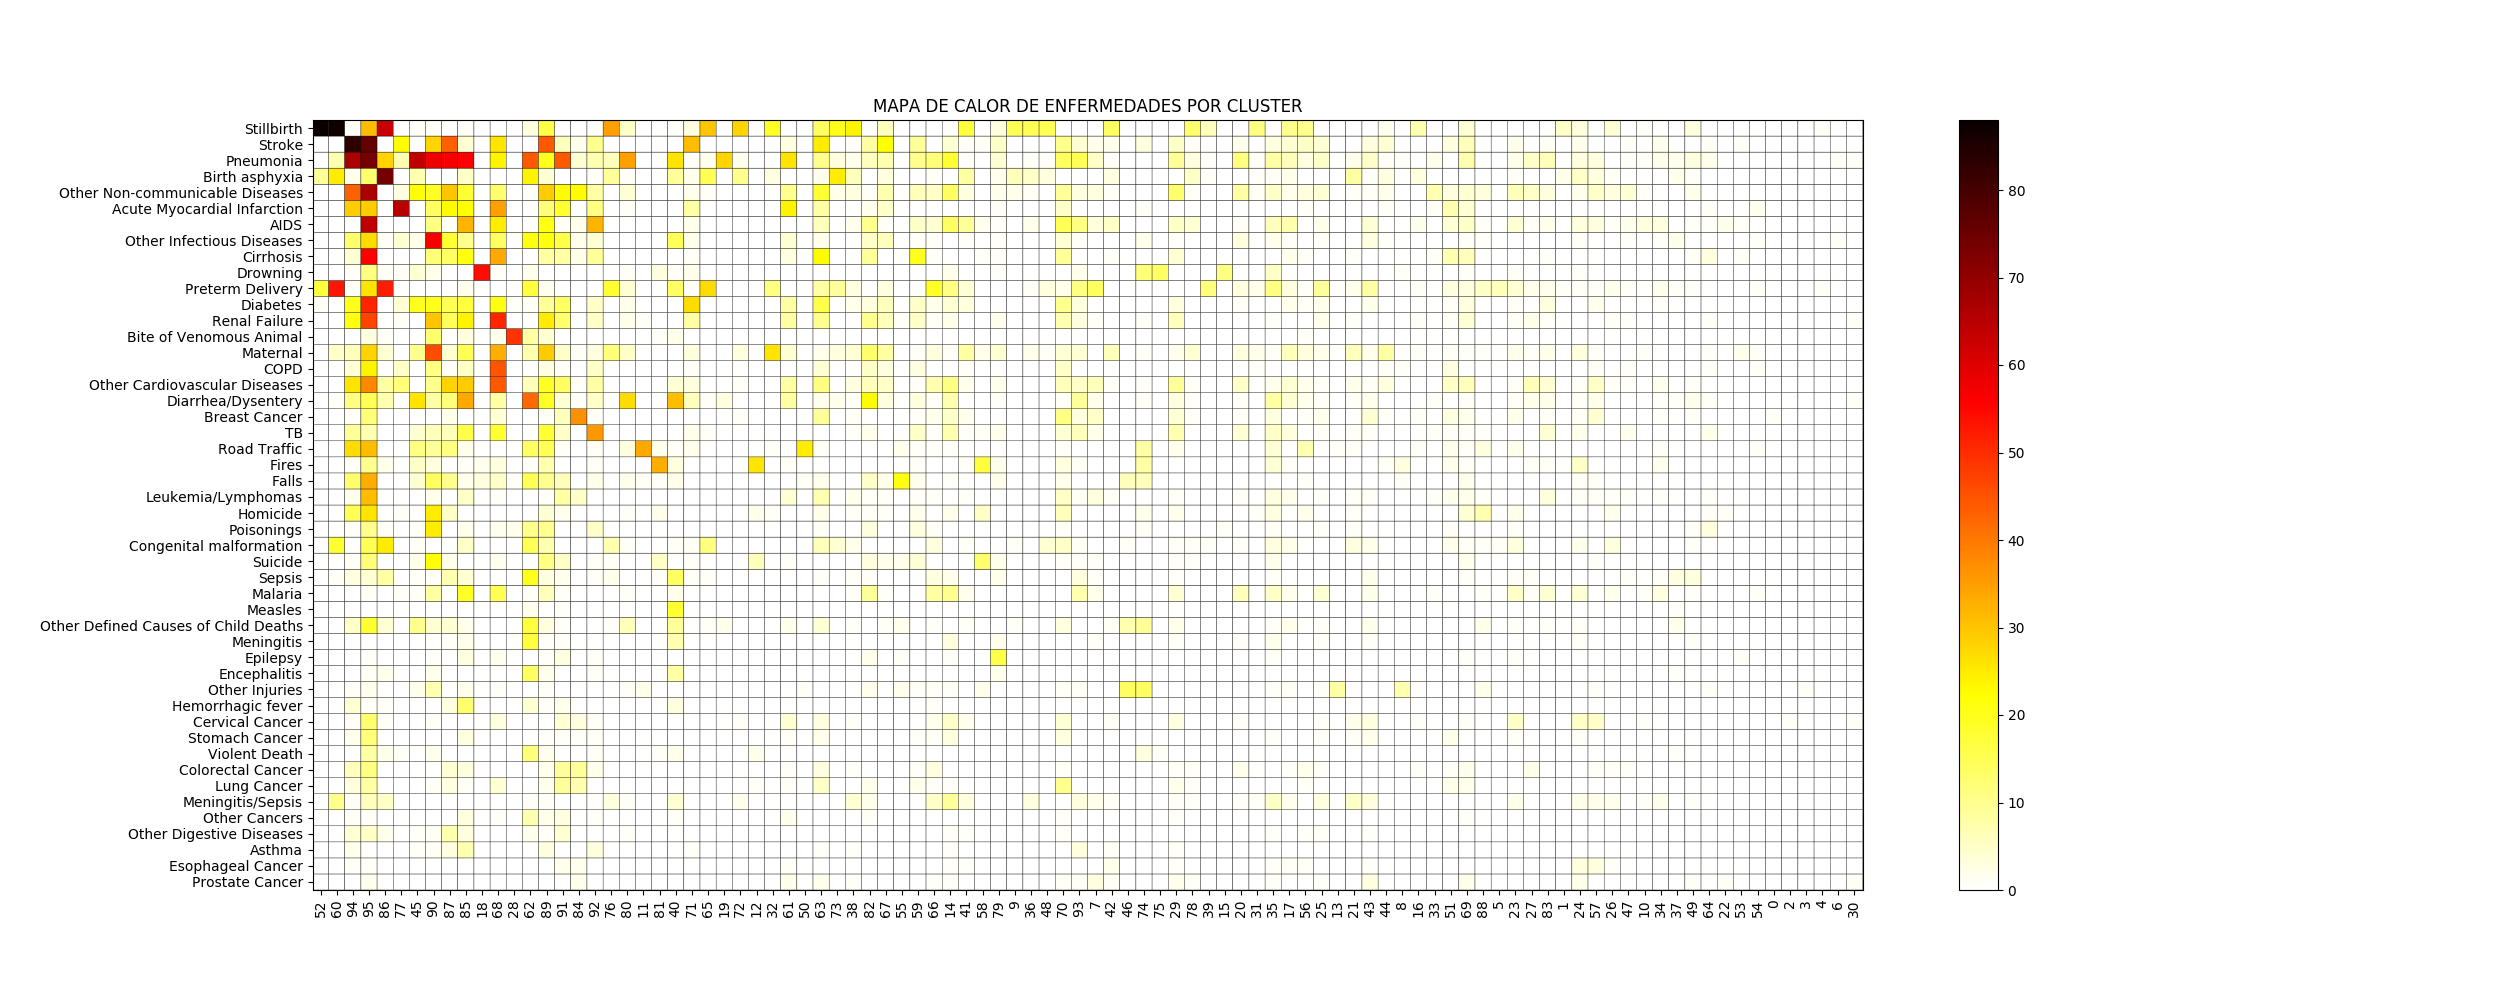
\includegraphics[width=\paperwidth]{figures/heatmap_k96_m2_init2k.png}}
		\caption{Heatmap (k=96, m=2, init=2k)}
		\label{fig:htm_96_2_2k}
	\end{figure}
	\paragraph{}
	Parece que al iniciar el clustering con centroides más separados entre sí, las distribución de instancias ha sido menos uniforme, haciendo que algunos clusters sean más densos y que otros lo sean menos en comparación a la inicialización aleatoria. Por esta razón, la relación entre los clusters y las clases está menos definida. Esto también se ve comparando el heatmap de la inicialización 2k (Fig: \ref{fig:htm_96_2_2k}) con el de la inicialización aleatoria (Fig: \ref{fig:htm_96_2_random}).
	
	\subsubsection{Distancia Minkowski}
	Por último, probamos a variar el parámetro $m$ de la distancia Minkowski y elegimos los valores 2 y 4. El resultado de utilizar $m=4$ es un el error total de los clusters (Fig: \ref{fig:sse_96_4_random}) ligeramente más alto en comparación a la misma operación realizada con $m=2$ (Fig: \ref{fig:sse_96_2_random}). Sin embargo, comparando los mapas de calor (Fig: \ref{fig:htm_96_2_random} y \ref{fig:htm_96_4_random}), parece que $m=4$ hace un trabajo ligeramente mejor de segregar las instancias según su clase.
	
	\begin{figure}
		\centering
		\makebox[\columnwidth]{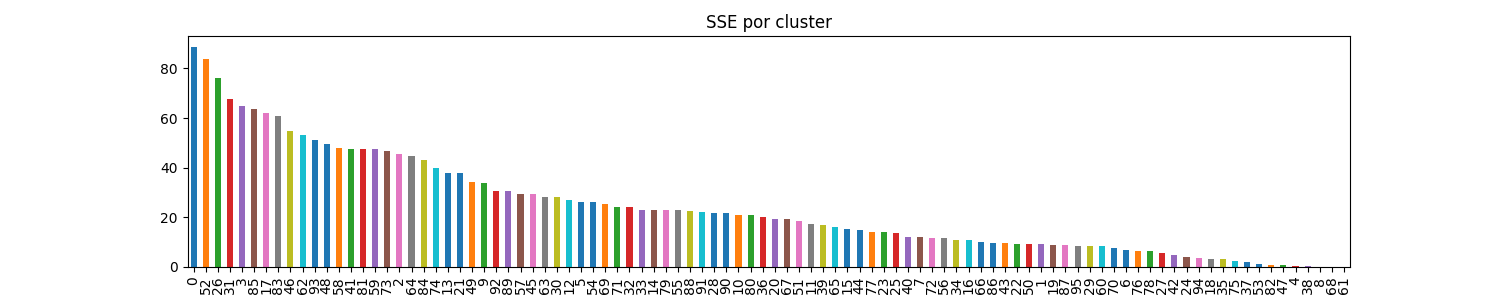
\includegraphics[width=\paperwidth]{figures/sse_plot_k96_m4_initrandom.png}}
		\caption{SSE por cluster(k=96, m=4, init=random)}
		\label{fig:sse_96_4_random}
	\end{figure}	
	\begin{figure}
		\centering
		\makebox[\columnwidth]{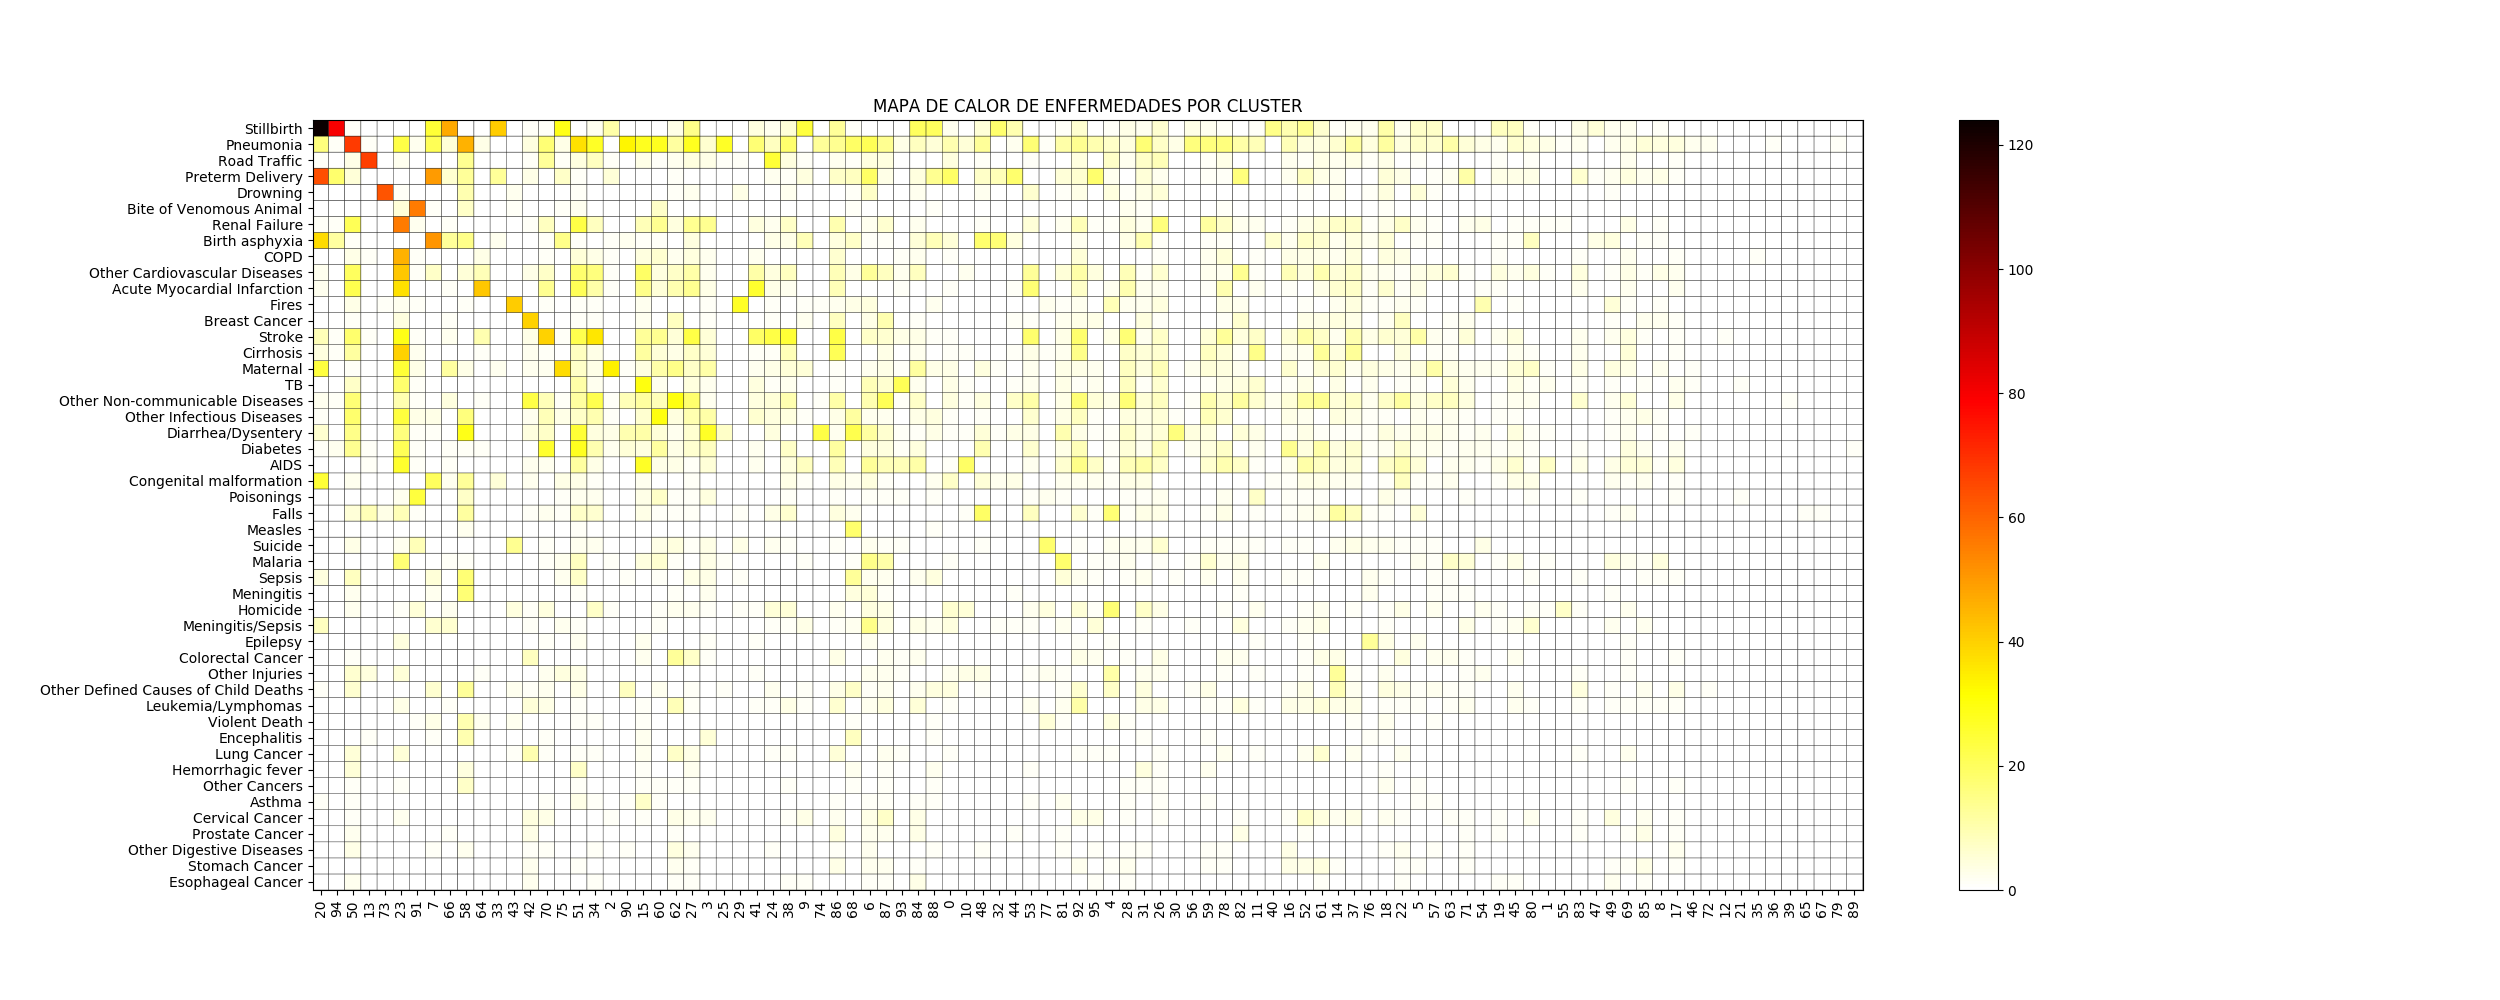
\includegraphics[width=\paperwidth]{figures/heatmap_k96_m4_initrandom.png}}
		\caption{Heatmap (k=96, m=4, init=random)}
		\label{fig:htm_96_4_random}
	\end{figure}
	
\section{Conclusiones}
	%Describir muy brevemente la motivación para llevar a cabo técnicas de clustering
	\paragraph{}
	Gracias a este proyecto hemos podido ver de primera mano una de las posibles aplicaciones de las técnicas de clustering. Hemos de tener en cuenta que es una técnica ampliamente utilizada en el mundo empresarial y laboral a unas escalas que no son comparables a nuestro pequeño proyecto, pero éste sirve como una buena aproximación a un mundo que todavía está en auge y en el que aún no hay muchas normas impuestas. 
	%Conclusiones generales (análisis de fortalezas del software implementado y reflexiones más importantes sobre la tarea)
	\paragraph{}
	En general nuestro programa cumple satisfactoriamente con los objetivos propuestos. Hemos sido capaces de desarrollarlo de forma que sea lo más potente, versátil y eficiente posible. Han sido estos dos últimos de especial importancia para nuestro grupo, puesto que por un lado la versatilidad nos ha permitido realizar pruebas con diferentes escenarios y parámetros para poder buscar fácilmente la mejor opción de clustering, y por otro lado hemos tenido que hacer nuestro código lo más eficiente posible ya que ha habido que realizar una gran cantidad de operaciones sobre un conjunto de datos de por si bastante grande, y en las primeras iteraciones del programa los ordenadores menos potentes del grupo no eran capaces de realizar estas tareas correctamente. Esto fue corregido posteriormente, consiguiendo que con el código final se pueda realizar la tarea en tiempos bastante bajos para la magnitud de ésta.
	%Propuestas para mejorar o ampliar la funcionalidad del software diseñado en trabajo futuro (análisis de puntos débiles y propuesta para solucionarlos)
	\paragraph{}
	Sin embargo, si tuviésemos que mejorar nuestro software una de las cosas en las que podríamos centrarnos es en dividir las instancias de forma previa al clustering en función de ciertos parámetros que hacen que estas instancias no sean completamente homogéneas. Un claro ejemplo de esto son los rangos de edad con los que están etiquetadas las instancias, en los que podemos ver que para aquellas instancias catalogadas como neonatos el abanico de causas de muerte es muy reducido. Otro posible ejemplo es el sexo de cada una de las personas, ya que es posible que no se pueda padecer alguna enfermedad según éste (un claro caso sería un cáncer testicular), o simplemente influir mucho en el conjunto de enfermedades que le pueden afectar. En ambos casos podría ser muy interesante disponer de la funcionalidad de realizar un clustering por separado.
	\paragraph{}
	Otro de las posibles áreas de mejora tiene que ver con los parámetros que nuestro algoritmo utiliza, tales como el número de clusters, el orden de la distancia de Minkowski, o la inicialización de los clusters. En este momento todos estos valores son introducidos por el usuario y, si bien eso añade versatilidad a nuestro programa, podría ser el propio programa el que ofreciese la posibilidad de probar con diferentes valores y ofrecer al usuario la mejor solución que pueda encontrar.
\section{Bibliografía}
\def\section*#1{} %Elimina el título "Referencias".
\bibliographystyle{unsrtnat}
\begin{thebibliography}{}

\bibitem{Minkowski} 
Binbin Lu et Al., The Minkowski approach for choosing the distance metric in geographically weighted regression, International Journal of Geographical Information Science, 2015

\bibitem{AliciaPerez} 
Alicia Pérez, Tema 2: CLUSTERING, UPV/EHU Bilbao, 10 Septiembre 2018

\end{thebibliography}

\end{document}
